\documentclass[11pt]{article}
\usepackage[margin=1.05in]{geometry}
\usepackage{amsmath,amssymb,bm}
\usepackage{booktabs}
\usepackage{siunitx}
\usepackage{graphicx}
\usepackage{tikz}
\usetikzlibrary{arrows.meta,positioning,fit,backgrounds}
\usepackage{listings}
\usepackage{xcolor}
\usepackage[colorlinks=true,linkcolor=blue,citecolor=blue,urlcolor=blue]{hyperref}

\newcommand{\ud}{\,\mathrm{d}}
\newcommand{\vect}[1]{\bm{#1}}
\newcommand{\file}[1]{\texttt{#1}}

\lstset{basicstyle=\ttfamily\footnotesize, frame=single, framesep=4pt,
        backgroundcolor=\color{gray!6}, columns=fullflexible,
        breaklines=true, showstringspaces=false}

\tikzset{
  stage/.style={draw, rounded corners=2pt, align=center, font=\small,
                minimum height=8mm, inner xsep=5pt, fill=blue!5},
  opt/.style={stage, fill=gray!8, densely dashed},
  data/.style={draw, align=center, font=\scriptsize\ttfamily, fill=yellow!10,
               minimum height=7mm, inner xsep=4pt},
  fl/.style={-{Stealth[length=2mm]}, thick},
}

\title{GTO $\to$ South-Pole Tulip: \\
Problem, Formulation, Discretization, and How to Run It}
\author{Michael Casey}
\date{July 26, 2026}

\begin{document}
\maketitle

\begin{abstract}
A working guide to the direct (collocation) solution of the minimum-fuel
low-thrust transfer from GTO to a south-pole \emph{tulip} orbit in the
Earth--Moon circular restricted three-body problem. It states the transfer
problem and its optimal control problem, derives why the discretization uses a
Sundman-regularized mesh with a fixed final pseudo-time, walks the solution
pipeline stage by stage, and documents how to run the code and how to tell
whether the answer should be believed. It is deliberately a \emph{guide}: the
derivations behind the method live in the companion notes
(\file{sundman\_minfuel\_solution\_note}, \file{minfuel\_method\_note}), and
what is \emph{not} solved is stated as plainly as what is.
\end{abstract}

\tableofcontents

%=======================================================================
\section{The transfer problem}
%=======================================================================

A \SI{15}{\kilo\gram} spacecraft with a \SI{25}{\milli\newton} electric
thruster ($I_{sp}=\SI{2100}{\second}$) departs a geostationary transfer orbit
and must rendezvous with a south-pole tulip orbit in the Earth--Moon system.
Thrust-to-weight is small enough that the transfer is a spiral of roughly forty
revolutions, not a two-impulse manoeuvre, and the Moon's gravity is a
first-order participant rather than a perturbation --- so the dynamics are
posed in the circular restricted three-body problem (CR3BP), in the rotating
frame, non-dimensionalized on the Earth--Moon distance $l^\ast$ and time
$t^\ast$.

Two numbers anchor everything downstream:

\begin{center}
\begin{tabular}{lll}
\toprule
quantity & value & where it comes from \\
\midrule
$t_{f,\min}$ & $6.290694$ ND $=\SI{27.8845}{\day}$ & certified min-time solution \\
flagship $t_f$ & $1.15\,t_{f,\min}=\SI{32.07}{\day}$ & the certified min-fuel row \\
\bottomrule
\end{tabular}
\end{center}

Transfer times are quoted throughout as the \emph{factor} $t_f/t_{f,\min}$.
The minimum-time solution is the anchor because minimum-fuel is only
interesting for $t_f>t_{f,\min}$: below that the problem is infeasible, and
just above it the coast arcs vanish and the answer degenerates to the
all-burn min-time solution.

%=======================================================================
\section{The optimal control problem}
%=======================================================================

\subsection{State, dynamics, control}

Let $\vect{r},\vect{v}\in\mathbb{R}^3$ be position and velocity in the rotating
frame and $m$ the mass. With $\mu^\ast$ the CR3BP mass parameter, $r_1,r_2$ the
distances to Earth and Moon, $T_{\max}$ the maximum thrust and $c$ the
effective exhaust velocity (all non-dimensional), the dynamics are
\begin{align}
\dot{\vect{r}} &= \vect{v}, \\
\dot{\vect{v}} &= \underbrace{-2\,\vect{\omega}\times\vect{v}
   - \vect{\omega}\times(\vect{\omega}\times\vect{r})}_{\text{rotating frame}}
   \;-\;\frac{(1-\mu^\ast)}{r_1^3}\vect{r}_1
   \;-\;\frac{\mu^\ast}{r_2^3}\vect{r}_2
   \;+\;\frac{T_{\max}}{m}\,s\,\vect{\alpha}, \\
\dot{m} &= -\frac{T_{\max}}{c}\,s .
\end{align}
The control splits into a \emph{throttle} $s\in[0,1]$ and a unit
\emph{direction} $\vect{\alpha}$, $\|\vect{\alpha}\|=1$. Boundary conditions
pin both endpoints: $(\vect{r},\vect{v})(0)=(\vect{r}_0,\vect{v}_0)$ on GTO and
$(\vect{r},\vect{v})(t_f)=(\vect{r}_f,\vect{v}_f)$ on the tulip, with $m(0)$
given and $m(t_f)$ free. Both endpoint states come from one place in the code,
\file{insertion\_states.m}, so that every pipeline in the repository starts and
ends at literally the same numbers.

\subsection{Objective, and why it is solved through a homotopy}

Minimum fuel means maximum final mass, i.e.
\begin{equation}
J_{\text{fuel}} \;=\; \int_0^{t_f} s(t)\ud t
\qquad\longrightarrow\qquad \min .
\label{eq:Jfuel}
\end{equation}
This is \emph{linear} in $s$. Pontryagin's minimum principle therefore gives a
bang--bang throttle governed by a switching function $S$: $s=1$ where $S<0$,
$s=0$ where $S>0$, with singular arcs only where $S\equiv0$ on an interval. For
a forty-revolution spiral the optimal control has on the order of twenty-five
switches, and a nonlinear program handed \eqref{eq:Jfuel} directly must
discover all of them at once from a cold start. It does not.

The fix is the Bertrand--\'Epenoy energy-to-fuel homotopy: solve instead
\begin{equation}
J(\varepsilon) \;=\; \int_0^{t_f}\Big[\,s - \varepsilon\, s(1-s)\,\Big]\ud t ,
\qquad \varepsilon: 1 \to 0 .
\label{eq:homotopy}
\end{equation}
At $\varepsilon=1$ the integrand is $s^2$ --- the \emph{minimum-energy} problem,
strictly convex in the control, smooth, and with a large basin of attraction.
At $\varepsilon=0$ it is exactly \eqref{eq:Jfuel}. Sweeping $\varepsilon$
downward and warm-starting each solve deforms a smooth solution continuously
into the bang--bang one, letting the switching structure emerge a few switches
at a time instead of all at once.

\emph{This single parameter is the campaign's main dial.} In the code it is
\texttt{epsMin}: set it to $1$ for a minimum-energy answer, $0$ for
minimum-fuel, anything between for a partially sharpened
($\varepsilon$-optimal) control.

%=======================================================================
\section{Discretization}
%=======================================================================

\subsection{Sundman regularization, and why not time}

Discretized uniformly in time, this problem fails for a structural reason: near
perigee the spacecraft moves fast and the gravity gradient
($\sim 1/r_1^3$) is enormous, so a mesh fine enough near perigee is
extravagantly wasteful over the rest of each revolution --- and one coarse
enough elsewhere cannot resolve perigee at all. Across forty revolutions this
is fatal.

The remedy is to change the independent variable from time $t$ to a
pseudo-time $\tau$ through the Sundman transformation
\begin{equation}
\frac{\ud t}{\ud \tau} \;=\; \kappa \;=\; r_1^{\,p},
\qquad p = 1.5 ,
\end{equation}
carrying time as an eighth state $t(\tau)$. Because $\kappa$ shrinks near
Earth, a \emph{uniform} $\tau$ grid automatically concentrates nodes at
perigee, exactly where they are needed, and the $1/r_1^3$ terms in the
$\tau$-domain Hessian are tamed.

\subsection{Fixed $\tau_f$, and how $t_f$ is then enforced}

A subtlety worth stating because it looks like a limitation and is in fact a
deliberate trade. The final pseudo-time $\tau_f$ is held \textbf{fixed}. If
$\tau_f$ were a free decision variable it would couple to every node, producing
a dense column in the KKT matrix; at $N\approx4000$ nodes the sparse
factorization (MUMPS) then exhausts memory. Holding $\tau_f$ fixed keeps the
KKT matrix banded.

The physical transfer time is instead enforced as a terminal condition on the
time state,
\begin{equation}
t(\tau_f) \;=\; t_f ,
\end{equation}
which is a single scalar constraint and costs nothing structurally. The price
is paid elsewhere, and it is the campaign's main open problem: with $\tau_f$
fixed the winding number of the trajectory cannot grow, so a solution cannot be
continued to a regime that needs \emph{more} revolutions (see
\S\ref{sec:open}).

\subsection{The nonlinear program}

Trapezoidal collocation on a uniform $\tau$ grid $\{\tau_k\}_{k=0}^{N}$ with
$h=\tau_{k+1}-\tau_k$ gives defect constraints
\begin{equation}
\vect{x}_{k+1}-\vect{x}_k-\frac{h}{2}\Big[\vect{f}(\vect{x}_{k+1},\vect{u}_{k+1})
+\vect{f}(\vect{x}_k,\vect{u}_k)\Big] \;=\; \vect{0},
\qquad k=0,\dots,N-1,
\end{equation}
with $\vect{x}=(\vect{r},\vect{v},m,t)\in\mathbb{R}^8$ and
$\vect{u}=(\vect{\alpha},s)\in\mathbb{R}^4$, plus $\|\vect{\alpha}_k\|=1$ and
$0\le s_k\le 1$ at every node, and the objective \eqref{eq:homotopy} evaluated
by the same trapezoidal quadrature. The flagship runs at $N=4001$ nodes:
roughly $48{,}000$ variables and $36{,}000$ equality constraints. It is
assembled and solved with CasADi + IPOPT, with exact sparse first and second
derivatives by algorithmic differentiation.

%=======================================================================
\section{The solution pipeline}
%=======================================================================

Figure~\ref{fig:pipeline} is the whole method. Only the first stage is
mandatory; everything after it is opt-in.

\begin{figure}[htbp]
\centering
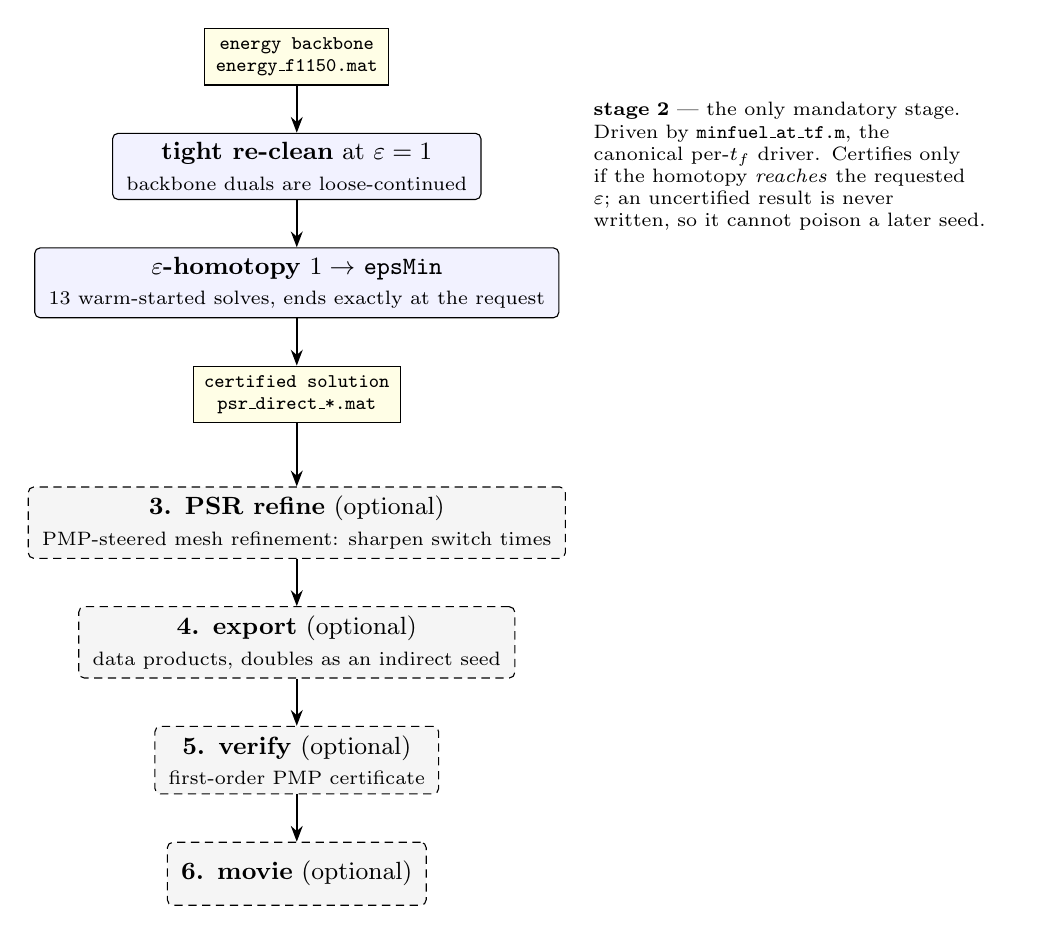
\begin{tikzpicture}[node distance=6mm]
  \node[data] (bb) {energy backbone\\ \file{energy\_f1150.mat}};
  \node[stage, below=of bb] (clean) {\textbf{tight re-clean} at $\varepsilon=1$\\
        \scriptsize backbone duals are loose-continued};
  \node[stage, below=of clean] (hom) {\textbf{$\varepsilon$-homotopy} $1\to$ \texttt{epsMin}\\
        \scriptsize 13 warm-started solves, ends exactly at the request};
  \node[data, below=of hom] (sol) {certified solution\\ \file{psr\_direct\_*.mat}};

  \node[opt, below=8mm of sol] (psr) {\textbf{3. PSR refine} (optional)\\
        \scriptsize PMP-steered mesh refinement: sharpen switch times};
  \node[opt, below=of psr] (exp) {\textbf{4. export} (optional)\\
        \scriptsize data products, doubles as an indirect seed};
  \node[opt, below=of exp] (ver) {\textbf{5. verify} (optional)\\
        \scriptsize first-order PMP certificate};
  \node[opt, below=of ver] (mov) {\textbf{6. movie} (optional)};

  \draw[fl] (bb) -- (clean);
  \draw[fl] (clean) -- (hom);
  \draw[fl] (hom) -- (sol);
  \draw[fl] (sol) -- (psr);
  \draw[fl] (psr) -- (exp);
  \draw[fl] (exp) -- (ver);
  \draw[fl] (ver) -- (mov);

  \node[right=13mm of clean, font=\scriptsize, align=left, text width=52mm]
      {\textbf{stage 2} --- the only mandatory stage.\\
       Driven by \file{minfuel\_at\_tf.m}, the\\
       canonical per-$t_f$ driver. Certifies only\\
       if the homotopy \emph{reaches} the requested\\
       $\varepsilon$; an uncertified result is never\\
       written, so it cannot poison a later seed.};
\end{tikzpicture}
\caption{The pipeline behind \file{run\_gto\_tulip.m}. Solid boxes are always
run; dashed boxes are opt-in stages. The energy backbone at the requested
$t_f$ is the entry point: it is the $\varepsilon=1$ root of the homotopy.}
\label{fig:pipeline}
\end{figure}

\paragraph{Where the seed comes from.} The homotopy needs a starting point at
$\varepsilon=1$. That is the \emph{energy backbone}: a converged minimum-energy
solution at the same $t_f$, banked under
\file{results/energy/energy\_f\#\#\#\#.mat}. Backbones exist for factors
$1.12$--$1.95$. Alternatively a neighbouring \emph{solved} bang--bang solution
can seed a nearby $t_f$ (\texttt{seedSpec = 'neighbor'}), which is far cheaper
because the switching structure is already present --- this is how the
$\Delta V$ versus $t_f$ front is walked.

%=======================================================================
\section{How to run it}
%=======================================================================

\subsection{One transfer}

\begin{lstlisting}[language=Matlab]
cd orbit_transfer/GTO_tulip/direct
setup_paths                 % the one path setup for this campaign
edit run_gto_tulip          % set section 1, then run
\end{lstlisting}

\file{run\_gto\_tulip.m} is the single entry point. The parameters that matter:

\begin{center}
\begin{tabular}{lll}
\toprule
parameter & meaning & typical \\
\midrule
\texttt{factor}   & $t_f/t_{f,\min}$                       & \texttt{1.15} \\
\texttt{epsMin}   & homotopy endpoint: 1 energy, 0 fuel     & \texttt{0} \\
\texttt{seedSpec} & \texttt{'energy'} $\mid$ \texttt{'neighbor'} $\mid$ path & \texttt{'energy'} \\
\texttt{insertion}& tulip insertion criterion               & \texttt{'campaign'} \\
\texttt{doRefine} & run the optional PSR stage              & as wanted \\
\texttt{movieMode}& \texttt{'none'} $\mid$ \texttt{'preview'} $\mid$ \texttt{'movie'} & \texttt{'none'} \\
\bottomrule
\end{tabular}
\end{center}

Stages are resumable: each skips itself when its output already exists, so a
re-run continues rather than restarting. Artifacts land in \file{results/}
(solver products, caches) and \file{data/} (exported data products).

\subsection{Sweeping the $\Delta V$--$t_f$ front}

\begin{lstlisting}[language=bash]
./run_tulip_front.sh              # default band, minimum fuel
./run_tulip_front.sh 1.15 1.20    # only these factors
EPSMIN=1 ./run_tulip_front.sh     # a minimum-energy sweep instead
\end{lstlisting}

Each factor runs in its own MATLAB process (crash isolation), the sweep is
resumable, and a failed factor is recorded rather than fatal --- an
uncertified factor is information about the front, not a reason to stop.

\paragraph{Why this sweeps $t_f$ and not thrust.} The sibling campaigns
(\file{earth\_elliptic\_to\_geo}, \file{earth\_elliptic\_to\_geo\_CR3BP}) sweep
\emph{thrust}, because thrust is the dimension that works for them. For the
tulip it is not; see \S\ref{sec:open}.

\subsection{Reproducing the flagship}

\begin{lstlisting}[language=Matlab]
best = run_certified_minfuel(1500, '/tmp/repro_check.mat');   % ~30 min
\end{lstlisting}

Pass an explicit save path: with no second argument this \emph{overwrites} the
published reference. Judge the result on mass and $\Delta V$, not on the switch
count --- see \S\ref{sec:certification}.

%=======================================================================
\section{What is certified, and what that means}
\label{sec:certification}
%=======================================================================

A run is called \emph{certified} when the homotopy reaches the requested
$\varepsilon$ endpoint with a solve that converged tight (IPOPT success status
and maximum defect below $10^{-6}$; in practice the flagship sits at
$\sim2\times10^{-14}$). An uncertified attempt is returned for inspection but
never saved.

That word is doing limited work, and the limits should be explicit:

\begin{itemize}
\item \textbf{It is a first-order, discrete statement.} The NLP satisfies its
own KKT conditions to tolerance. The generic first-order gate
(\file{verify\_common}) additionally checks the discrete costates against the
PMP conditions --- stationarity, the switching-function sign law,
transversality --- and \file{certify\_minfuel\_pmp.m} propagates the
state--costate system arc by arc as an independent check.

\item \textbf{Second-order optimality is not established.} The NLP SSOSC test
via KKT inertia is structurally inapplicable here, and the
Maurer--Osmolovskii switching-time Hessian is blocked by forward-flow
conditioning. What exists is an IPOPT native-inertia observation, which is
evidence, not proof. Status is tracked in
\file{orbit\_transfer/OPTIMALITY\_CERTIFICATION.md}.

\item \textbf{The switch count is not reproducible; the mass is.} Three
independent re-solves of the certified recipe (2026-07-21, and twice on
2026-07-26) all returned \textbf{24} switches against the published 25, with
final mass agreeing to $\sim0.1\%$. The switch integer is basin-sensitive even
at fixed mesh. Report it as a band.

\item \textbf{There are at least two certified optima at the flagship $t_f$.}
The energy-backbone route and the \file{run\_certified\_minfuel} chain both
converge machine-tight to 25 switches at the \emph{same} $t_f$ and land on
different local optima ($m_f = 0.847086$ versus $0.849066$; $\Delta V$
$3.4176$ versus \SI{3.3696}{\kilo\meter\per\second}). The seed route decides
which. Stage 2 prints a basin check against the reference so this cannot pass
unnoticed.
\end{itemize}

\begin{center}
\begin{tabular}{lS[table-format=2.0]S[table-format=1.6]S[table-format=1.4]S[table-format=1.4]}
\toprule
route & {switches} & {$m_f$} & {$\Delta V$ (km/s)} & {prop (kg)} \\
\midrule
published flagship             & 25 & 0.849066 & 3.3696 & 2.2640 \\
energy backbone $\to$ homotopy & 25 & 0.847086 & 3.4176 & 2.2937 \\
re-solve, 2026-07-26           & 24 & 0.849279 & 3.3644 & 2.2608 \\
\bottomrule
\end{tabular}
\end{center}

%=======================================================================
\section{What is not solved}
\label{sec:open}
%=======================================================================

\paragraph{The near-minimum-time band, $1.01 \le t_f/t_{f,\min} \le 1.11$.}
No certified solution exists there, and the obstruction is not the bang--bang
structure: the \emph{smooth} minimum-energy backbone itself will not converge
in that band. It is a conditioning wall approaching minimum time, where coast
arcs shrink toward zero measure. The front therefore starts at $1.12$.

\paragraph{The thrust ladder.} Off-nominal thrust is not merely untested, it is
blocked. Chaining the certified \SI{25}{\milli\newton} solution to
\SI{20}{\milli\newton} at the same factor fails at the $\varepsilon=1$ energy
step: a lower-thrust rung needs \emph{more} revolutions, and with $\tau_f$
fixed (\S3.2) the winding number of a chained seed cannot grow. This is a
topology wall, not a tuning problem, and escaping it needs a free-span
reformulation ($\Delta\theta$-free, the analogue of the MEE campaigns' free
longitude span). \file{run\_gto\_tulip} therefore \emph{refuses} off-nominal
thrust with that explanation rather than running a solve expected to fail.

\paragraph{Indirect certification.} The indirect campaigns
(\file{indirect/ms\_band}, \file{ifs}, \file{ztl}) have working machinery but
no certified indirect solve of this problem.

%=======================================================================
\section{Where things live}
%=======================================================================

\begin{center}
\begin{tabular}{ll}
\toprule
path & contents \\
\midrule
\file{direct/run\_gto\_tulip.m} & the front door (six stages) \\
\file{direct/lib/}      & solver, homotopy, seeds, refinement algorithm \\
\file{direct/certify/}  & PMP verification, second-order machinery, front aggregation \\
\file{direct/viz/}      & movies and frames \\
\file{direct/tests/}    & guardrail tests (seconds, no solves) \\
\file{direct/results/}, \file{direct/data/} & artifacts \\
\file{indirect/}        & PMP shooting campaigns (ms\_band, ifs, ztl, min\_time) \\
\bottomrule
\end{tabular}
\end{center}

\paragraph{Companion documents.}
\file{doc/sundman\_minfuel\_solution\_note} derives the Sundman formulation and
the homotopy in full; \file{doc/minfuel\_method\_note} covers the method;
\file{process/LOW\_THRUST\_MINFUEL\_CAMPAIGN.md} is the campaign record ---
every method generation, what failed, and why;
\file{process/HONEST\_EVALUATION\_DV\_TF\_FRONT.md} assesses what the
certification does and does not prove.

\paragraph{A note on verification after structural changes.} The fast tests in
\file{direct/tests/} run in seconds and are worth running constantly, but they
do \emph{not} prove the campaign still works: after the 2026-07-26
restructure every one of them passed while the flagship reproduction was
broken by a single stale artifact path. \file{test\_artifact\_paths.m} now
catches that class in seconds, but the reproduction remains the ground truth.

\end{document}
